\documentclass[12pt]{article}
\usepackage[left=15mm,top=0.5in,bottom=0.5in,centering]{geometry}
\usepackage{listings}
\usepackage{framed}
\usepackage{graphicx}
\usepackage{wrapfig}
\usepackage{floatrow}
\usepackage{subfigure}
\usepackage{color}
\usepackage{amsmath}
\usepackage{lipsum}
\usepackage{hyperref}
\usepackage{amssymb}
\usepackage{rotating}
\usepackage{tikz}
\usepackage{tabu}
\usepackage{titlesec}
%\usepackage{algorithm}
\usepackage[linesnumbered,ruled,vlined,english,onelanguage]{algorithm2e}
%\usepackage{algorithmic}
\usepackage[noend]{algpseudocode}
\definecolor{dkgreen}{rgb}{0,0.6,0}
\definecolor{gray}{rgb}{0.5,0.5,0.5}
\definecolor{mauve}{rgb}{0.58,0,0.82}
\lstset{frame=tb,
	language=Java,
	aboveskip=3mm,
	belowskip=3mm,
	showstringspaces=false,
	columns=flexible,
	basicstyle={\small\ttfamily},
	numbers=none,
	numberstyle=\tiny\color{gray},
	keywordstyle=\color{blue},
	commentstyle=\color{dkgreen},
	stringstyle=\color{mauve},
	breaklines=true,
	breakatwhitespace=true,
	tabsize=3
}
\newcounter{question}
\setcounter{question}{0}
\def\thequestion{{\bf{Question \arabic{question}. }}\space }
\newcommand{\Question}[1]{\pagebreak \stepcounter{question}\noindent\thequestion#1\par}
\newcounter{countpart}[question]
\setcounter{countpart}{0}
\def\thepart{\\ \par (\alph{countpart}) \space}
\newcommand{\Part}[1]{\stepcounter{countpart}\noindent\thepart#1\normalfont{}}
\newenvironment{Parts}{\par\medskip
	\noindent \rmfamily}{\medskip}

\def\BeginSolution{\begin{framed}\noindent \normalfont{}}
	\def\EndSolution{\end{framed}\pagebreak}
\newcommand{\mat}[1]{\mathbf{#1}}
\newcommand{\matG}[1]{\boldsymbol{#1}}
\newcommand{\bm}[1]{\boldsymbol{#1}}
\def\real{\mathbb{R}}
\def\R{\mathbb{R}}
\newcommand{\norm}[1]{\left\lVert#1\right\rVert}
%\newcommand*\EE[1]{\ensuremath{\text{\textsc{e}}#1}}
\def\EE{\mathbb{E}}
\def\ev{\mathbb{E}}
\def\P{\mathbf{P}}
\def\y{\vec{y}}
\def\X{\mathbf{X}}
\def\x{\vec{x}}
\def\w{\vec{w}}
\def\b{\vec{b}}
\def\r{\vec{r}}
\def\T{^{\top}}
\def\argmin{\text{arg}\min\limits}
\def\argmax{\text{arg}\max\limits}
\def\I{\mathbb{I}}
\def\A{\vec{A}}
\def\tran{^{\top}}
\def\W{\mathbf{W}}
\def\z{\mathbb{z}}
\def\ell{l}
\newcommand{\diag}{\mathop{\mathrm{diag}}}
\allowdisplaybreaks
\usepackage[final]{pdfpages}
\setboolean{@twoside}{false}
\setcounter{MaxMatrixCols}{20}

\begin{document}
	\title{CS294-112 HW1\vspace{-2ex}}
	\author{Huanjie Sheng, 25928718\vspace{-2ex}}
	\date{\today \vspace{-2ex}}
	%\maketitle
	%\addcontentsline{toc}{subsection}{Appendices}
	%\renewcommand{\thesection}{(\arabic{section})}
	%\titleformat*{\subsection}{\normalfont}
	
	\section{Problem 4: Experiments}
	\subsection{Half Cheetah}
	Fig.\ref{fig:half_cheetah} shows that soft actor-critic (sac) can achieve very high return in half cheetah.  Using the reparametrization trick can increase the return even more than the REINFORCE algorithm.  This is because reparameterization tricks allows for better sampling which results in more accurate gradient estimation.
	\begin{figure}[!htbp] 
	 	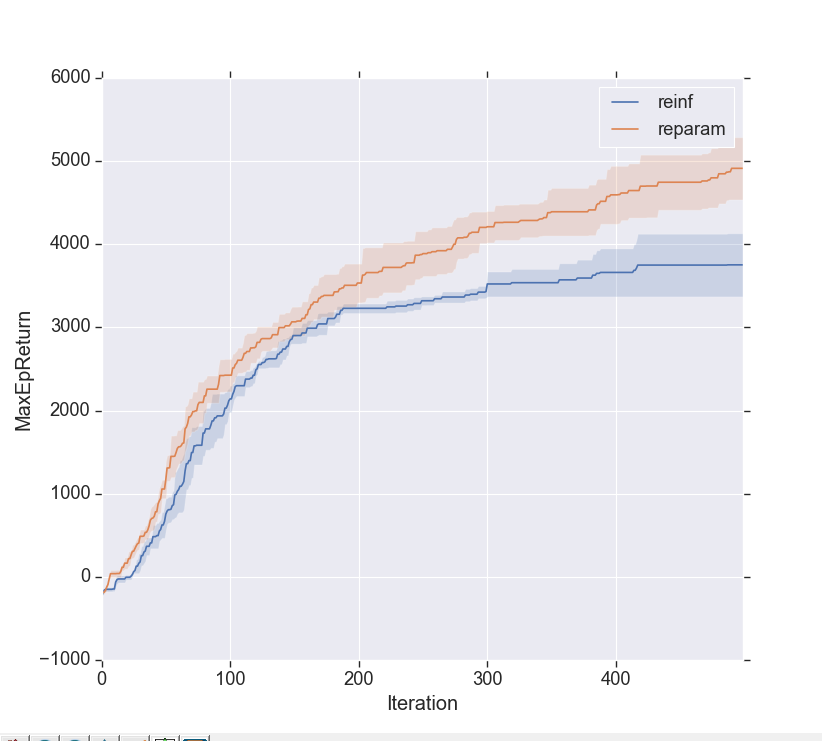
\includegraphics[width=1.0\textwidth]{figure_1.png}
	 	\caption[caption]{The performance of sac on half cheetah. \\ \hspace{0.4\textwidth}
	 	\textcolor{blue}{Blue}: the maximum expected return of REINFORCE algorithm,\\ \hspace{0.4\textwidth}
	 	\textcolor{orange}{Orange}: the maximum expected return using reparametrization trick.\label{fig:half_cheetah}}
	\end{figure}

	\pagebreak
	\subsection{Ant-v2}
	Fig.\ref{fig:ant_v2} shows that soft actor-critic (sac) can achieve very high return in Ant-v2 as well.  Using the two Q functions trick can increase the return a lot more.  This is because double Q learning decorrelates sample points allowing for better Q function and Value function estimations.
	\begin{figure}[!htbp] 
		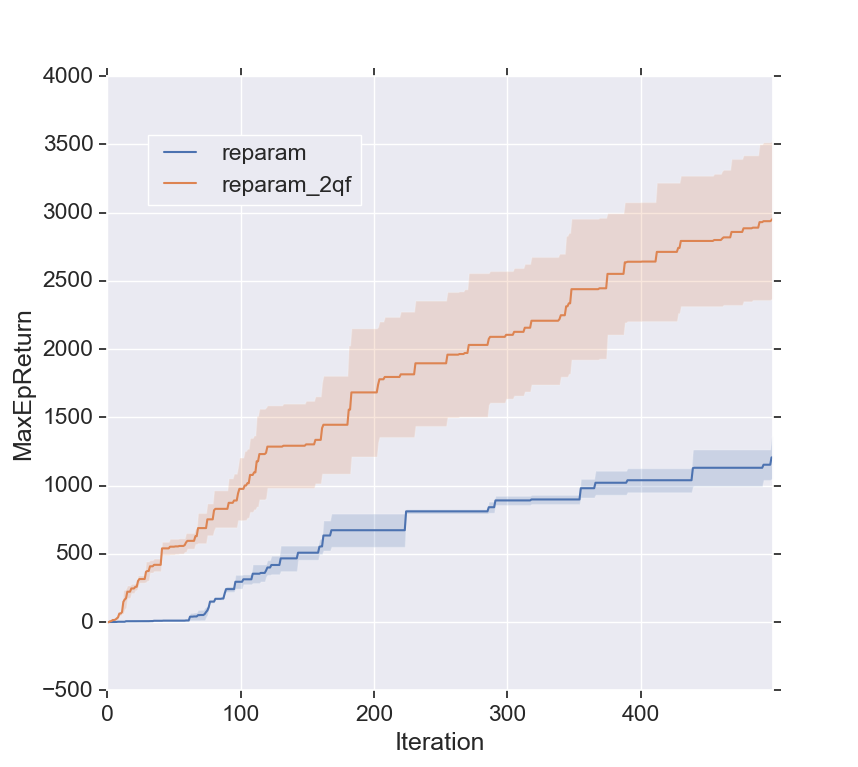
\includegraphics[width=1.0\textwidth]{figure_2.png}
		\caption[caption]{The performance of sac on Ant-v2. \\ \hspace{0.4\textwidth}
		\textcolor{blue}{Blue}: the maximum expected return with a single Q function using reparametrization trick,\\ \hspace{0.4\textwidth} \textcolor{orange}{Orange}: the maximum expected return with two Q functions using reparametrization trick.\label{fig:ant_v2}}
	\end{figure}
  
	
\end{document}